% !TEX TS?program = pdflatexmk
\documentclass[a4paper, 12pt, twoside]{article}
\usepackage[english]{babel}
\usepackage[utf8]{inputenc}
\usepackage[utf8]{inputenc}


%\renewcommand{\baselinestretch}{1.0} 
                    
                    
%Margins
\usepackage[left=25.4mm, right = 25.4mm, top=25.4mm, bottom=25.4mm, includefoot]{geometry}
%geometry{a4paper, total={170mm,257mm}, left=25.4mm, right = 25.4mm, top=25.4mm, bottom=25.4mm}
\setlength{\parindent}{0in}
\usepackage{enumitem}
       
                   
%Adding Pictures
\usepackage{graphicx}
\usepackage{float}
          
                    
%Header and Footers
\usepackage{fancyhdr}
\pagestyle{fancy}
\fancyhead{}
\fancyfoot{}
\fancyfoot[RO]{ Inspecting the Inspectors \hspace{1mm} \textbar \hspace{1mm} \thepage\ }
\fancyfoot[LE]{ \thepage \hspace{1mm} \textbar \hspace{1mm} DOING BUSINESS IN DELHI: A Compendium }
\renewcommand{\headrulewidth}{0pt} %change the pt width to insert header line
\renewcommand{\footrulewidth}{0pt} %change the pt width to insert footer line
\usepackage{amsmath}

            
                                      
%Tables
\usepackage{booktabs}
\usepackage{subfig}
\captionsetup{aboveskip=14pt,}
\captionsetup[table]{singlelinecheck = false}
\usepackage{array}
\newcolumntype{L}[1]{>{\raggedright\let\newline\\\arraybackslash\hspace{0pt}}m{#1}}
\newcolumntype{C}[1]{>{\centering\let\newline\\\arraybackslash\hspace{0pt}}m{#1}}
\newcolumntype{R}[1]{>{\raggedleft\let\newline\\\arraybackslash\hspace{0pt}}m{#1}}
\usepackage{makecell}	
\usepackage{multirow}
\usepackage{longtable}

%Lists
%\usepackage{enumerate}
%\usepackage{enumitem}
%\usepackage{alphalph}

                    
%Coloured Boxes
\usepackage{xcolor}
\usepackage{mdframed}
           
                    
%Symbols
\usepackage{pifont}
\usepackage{amssymb}
\newcommand{\cmark}{\ding{51}}%checkmark
\newcommand{\xmark}{\ding{55}}%xmark

%Custom Spacing
\usepackage{setspace}
         
                    
%Defining Colours
\definecolor{CCSbrown}{RGB}{163, 86, 37}
\definecolor{CCSgrey}{RGB}{105, 105, 105}
\definecolor{CCSblack}{RGB}{64, 64, 65} 
             
             
%Heading Colours                  
\usepackage{sectsty}
\usepackage{titlesec}
\chapterfont{\color{blue}}  %sets colour of chapters font
\sectionfont{\color{CCSbrown}}  %sets colour of section font
\subsectionfont{\color{CCSblack}} %sets colour of subsection font
\subsubsectionfont{\color{CCSblack}} %sets colour of subsubsection font
		
    				
%Bibliography
\usepackage[authordate, backend=biber]{biblatex-chicago}
\addbibresource{Labour.bib}
\usepackage{hyperref} %activates links 
\hypersetup{
colorlinks,
linkcolor = black,
citecolor = CCSbrown,
urlcolor = black}
\usepackage{blindtext}
\renewbibmacro*{cite:ibid}{\printtext[bibhyperref]{\bibstring[\mkibid]{ibidem}}} 		
              
\begin{document}

%==================================================

%Title Page
\begin{titlepage}
\begin{center}
\line(1,0){300}\\
[0.25in]
\huge{\bfseries\textcolor{CCSbrown} {Inspecting the Inspectors}} \\
[0.5cm]
\large{Mandate versus Reality Analysis of Labour \\Regulation Enforcement in Delhi} \\
    	
\line(1,0){200}\\
[3in]
\LARGE{Vatsal Bajaj, Shivani Pandey, and Aastha Sood} \\ 
[1.5cm]
%{\Large Centre for Civil Society} \\
{\normalsize New Delhi, India} \\
{\normalsize September 2018} \\
[2cm]

\includegraphics[width = 75mm]{CCSlogo.jpg}

\end{center}
\end{titlepage}

%=====================TOC==========================================================                 
\tableofcontents

%======================LIST OF ABBREVIATIONS======================================== 
\newpage
\newlist{abbrv}{itemize}{1}
\setlist[abbrv,1]{label=,labelwidth=1in,align=parleft,itemsep=0.1\baselineskip,leftmargin=!}

%List of Abbreviations         
\section*{List of Abbreviations}
\addcontentsline{toc}{section}{List of Abbreviations}

\begin{abbrv}
         
        \item[BRAP]			Business Reforms Action Plan
        \item[CRA]			Computerized Risk Assessment
        \item[DIPP]			Department of Industrial Policy and Promotion
        \item[EoDB]			Ease of Doing Business
        \item[ILO]				International Labour Organisation
        \item[GoNCT]			Government of National Capital Territory 
        \item[OECD]			Organisation of Economic Cooperation and Development
        \item[SOP]			Standard Operating Procedure 
              
\end{abbrv}

%=================EXECUTIVE SUMMARY==============================================
%Executive Summary
\newpage
\section*{Executive Summary}
\addcontentsline{toc}{section}{Executive Summary}

India has 44 central labour laws, which apply across the country, to promote and safeguard the interests of workers. In addition, states have their own labour laws and regulations. Labour inspectors at state labour departments in India monitor how these laws are applied in the workplace and are responsible for ensuring compliance by the employers, workers and worker unions. Over the years, discretionary powers vested in labour inspectors, lack of procedural clarity and opacity in the resolution process have harmed labour and enforcement and made the operating environment for businesses challenging. \\

In a bid to improve the ease of doing business (EoDB), Government of India’s Department of Industrial Policy and Promotion (DIPP) released the second iteration of the Business Reforms Action Plan (BRAP) in 2017. A segment of BRAP 2017 aimed to meet industry concerns around the ‘inspector raj’ in labour law enforcement and suggested six reforms in the functioning of state labour inspectorates as they enforce each labour law. These six reforms were aimed at reducing arbitrary powers assigned to the inspectorates and bringing transparency and consistency to labour inspections. The first of these asks state labour departments to publish information about the inspections procedure and a comprehensive inspection checklist on their website. \\

In its submission to the DIPP on the progress in the BRAP in October 2017, the Government of National Capital Territory (GoNCT) claims to have published, and by extension/inference, adopted the use of standard operating procedures (SOP) in the monitoring and enforcement of seven key labour laws under the purview of the Delhi Labour Department. As part of a larger research project on the EoDB in Delhi, we examine the claims of GoNCT on the implementation of SOPs in the inspections conducted by the Delhi Labour Department.\footnote{Throughout this research, we have referred to the state of Delhi as ‘Delhi’ and to the New Delhi district as ‘New Delhi’.} \\

We studied the administrative records of nearly 850 labour complaint entries received at the New Delhi district labour office, one of the nine inspectorates of the Delhi Labour Department. Through our analysis, we found several discrepancies in the use of SOPs to schedule, manage and conduct inspections in the labour inspection set-up in Delhi. To our knowledge, this is the first study that systematically looks at administrative data from complaint registers and case files to understand procedural hygiene in complaint resolution. \\

While SOPs have been published on the website of the Department, they are likely not being met with rigor. Indifferent, haphazard and nonstandardised record keeping, missing procedural hygiene and lack of fidelity to prescribed timelines are three nontrivial departures from SOPs. \\

First, we find that 98\% of the entries in the complaint registers had at least one missing field of information. For example, 92\% of the entries did not mention the Labour Act under which the complaint was registered, a crucial determinant of the SOP to be followed. Such inconsistent record keeping restricts the government from tracking progress, allocating manpower, and providing documentation that is beyond reproach in case of a legal challenge. \\

Second, our investigation into the records highlighted that missing definitions were making the lines between on-site inspections and in-office hearings blurry. Currently, SOPs for inspecting violations of the Minimum Wage Act and Payment of Bonus Act do not require on-site observations, but it is not clear how the inspectorate resolves these complaints. In addition, even for complaints registered under the Acts that do require on-site observations, we found no proof that on-site inspections were ever conducted. \\

Third, we find that timelines prescribed in SOPs are not being met. More than a third of the inspections from 2016 to 2018 were not conducted within 15 days after the receipt of complaints as prescribed. In addition, the high number of cases pending resolution may be highlighting a deeper malaise as more than half the complaints on the books remain unsettled nearly a year on. \\

Our interviews with Delhi Labour Department officials and complainants corroborate some of these concerns. Our interviews indicate that labour inspectors are unaware of crucial provisions of the labour laws and may not be applying SOPs correctly. Simultaneously, 60\% of complainants are dissatisfied with the redressal system for reasons ranging from excessive time taken for complaint resolution to proximity between the management and the inspector. \\

A catch-all explanation in our interviews with department officials is a shortage of manpower in the department. However, an analysis of the workload of New Delhi District Labour Office does not bear this out. On average, inspectors receive one complaint a day and more than 90\% of complaints can be resolved without conducting an on-site inspection. In such a situation, it is unclear why inspectors claim to be overburdened. We argue that poor procedural hygiene such as blurry lines between on-site inspections and in-office hearings and low levels of awareness among inspectors about the laws are perhaps more significant to complainant dissatisfaction, high pendency and a continued poor reputation. \\

In this study, we first outline the evolution of labour law enforcement in Delhi from suo-moto inspections to a complaint-based inspection system. Second, we describe the procedure for labour inspections as outlined under the SOPs for seven key laws. Third, we report the differences between mandate and practice in the current labour inspection system in New Delhi. This is based on an analysis of departmental administrative data, including complaints data, from the New Delhi District Labour Office and interviews with complainants and labour inspectors. Finally, we conclude. \\


%=================INTRODUCTION===================================================
\newpage
\section{Introduction}

Labour laws uphold provisions related to hours of work, wages, safety, health and welfare of persons employed as labour, as well as the employment of children. Strong labour laws can, in theory, lead to better working conditions, EoDB and a path to development (\cite{deshingkarpaper}).\\

In the seven decades since Independence, India has passed numerous labour laws that address core standards of worker health, safety and protection from injustices as specified by the International Labour Organisation (ILO). The first law enacted in India for the protection of workers’ rights was the Trade Unions Act, 1926. This was followed by the Factories Act, 1940. Other labour laws such as the Delhi Shops and Establishments Act, 1954, Contract Labour (Regulation And Abolition) Act, 1970, and the Payment of Gratuity Act, 1972, came into force post-independence. At present, there are 44 central labour laws and one state labour law governing employers and employees in Delhi. The subject of labour is in the concurrent list of the Constitution of India. This gives power to both the state and the central governments to enact legislations for the workforce.\footnote{See Appendix 1 for a list of all labour laws in force in Delhi.}\\

Over the years, a labour inspection system was formed to ensure compliance to the comprehensive legal structure for labour welfare and protection in India. Labour inspectorates have been set up at the state level to ensure that these labour laws are upheld. Deshingkar (\cite{deshingkarpaper}), however, finds that ‘despite having one of the most comprehensive labour legislative frameworks in the world, India continues to suffer from the widespread violation of labour laws’. \\

Inspections are the most visible and important among regulatory enforcement activities (\cite{oecdinspections2}, 9). An efficient and effective labour inspections system can ensure both workers’ welfare and improved financial results through higher productivity \parencite{iloreportlabour}. \\

While labour inspections serve workers’ interests, they can be a serious hindrance in conducting business unless they follow prescribed procedures, and are transparent and based on the rule of law. Ensuring that inspections are carried out in a fair and accountable manner where employers are not harassed and employee complaints are duly addressed becomes a crucial part of the EoDB.\\

%Recommendations on Labour Inspection Reforms in Business Reform Action Plan 2017
\subsection{Recommendations on Labour Inspections Reforms in Business Reform Action Plan 2017}

In order to improve EoDB in India, the DIPP of the Ministry of Commerce and Industry released the BRAP.\footnote{The first iteration of the BRAP was released in 2015. However, we look at the most recent plan, i.e the BRAP 2017.} As of September 2018, Delhi ranked 23 out of a total of 34 states, having implemented a third of the reforms suggested under the BRAP 2017.\\

In light of the importance of cleaning up labour inspections, the BRAP 2017 of DIPP recommended six inspections reforms as applied to seven key labour laws: 
\begin{enumerate}
\item \textbf{Publish a well-defined inspection procedure and checklist on the website of the department:} This includes all applicable steps and process maps if available. The reform requires the State Labour Department to publish this information explicitly without referring to Acts or rules. This inspection checklist published on the website is to further contain the SOPs being followed by state labour departments in inspections pertaining to every Act. 
\item \textbf{Design and implement a system for computerised allocation of inspectors:} The inspector allocation system must be linked to the online application and approval system, and the approval authority should be able to allocate inspectors once applications are submitted either by jurisdiction or randomly. The inspector should also have an online workspace in the system where they can see their workflows and submit reports.
\item \textbf{Mandate online submission of inspection report within 48 hours to the Department.}
\item \textbf{Allow establishments to view and download submitted inspection reports of at least past two years:} The signed inspection reports of the last 2 years—signed either digitally or manually and scanned—should be made available for viewing and downloading by the user on the portal or the website. 
\item \textbf{Design and implement a system for identifying establishments that need to be inspected based on computerised risk assessment (CRA):} To reduce burden on limited inspectors and increase efficiency, inspectorates should define risk criteria and ensure that they are programmed into the system to make sure that inspections occur only for certain high-risk categories, instead of in 100\% of the applications.
\item \textbf{Mandate that the same inspector will not inspect the same establishment twice consecutively:} Inspectors should be assigned randomly for inspections in consecutive years in order to increase transparency and reduce the potential for corruption.
\end{enumerate}

%Progress of the Government of National Capital Territory in Implementing Labour Inspection Reforms 
\subsection{Progress of the Government of National Capital Territory in Implementing Labour Inspection Reforms}

Table 1 provides a summary of the progress of the GoNCT in implementing labour inspections reforms. The GoNCT on the website of DIPP website has claimed to have implemented the first. None of the five remaining recommendations have been \\implemented by Delhi. 

%Table 1: Labour Inspection Reforms Adopted by Delhi under the BRAP 2017
\begin{table}[H]
  \caption{Labour Inspection Reforms Adopted by Delhi under the BRAP 2017}
\begin{footnotesize}
    \begin{tabular}{p{3.5cm}p{4em}p{5.5em}p{5.1em}p{4.5em}p{3.5em}p{4.2em}}
\toprule
    Act to Which & \multicolumn{6}{p{30.33em}}{\centering Six Key Labour Inspection Reforms Under the BRAP 2017} \\
    the Reform Applies & \multicolumn{6}{p{31.33em}}{\footnotesize{(Nos. refer to the Specific Reform Item in the Implementation Guideline)}} \\
\midrule
    \multicolumn{1}{r}{} & Checklist    + SOP & Computerised Inspector Allocation & Online Submission Of Reports  & Remotely Accessible Reports  & CRA   & Unique Inspector Per Visit \\
\toprule
    Equal\\ Remuneration Act & \#116 \checkmark & \#117 \xmark & \#118 \xmark & \#119 \xmark & \#120 \xmark & \#121 \xmark \\
	&	&	&	&	&	& \\
    Minimum Wages Act & \#128 \checkmark & \#129 \xmark & \#130 \xmark & \#131 \xmark & \#132 \xmark & \#133 \xmark \\
	&	&	&	&	&	& \\
    Shops \& \\Establishment Act & \#134 \checkmark & \#135 \xmark & \#136 \xmark & \#137 \xmark & \#138 \xmark & \#139 \xmark \\
	&	&	&	&	&	& \\
    Payment of Bonus Act & \#140 \checkmark & \#141 \xmark & \#142 \xmark & \#143 \xmark & \#144 \xmark & \#145 \xmark \\
	&	&	&	&	&	& \\
    Payment of Wages Act & \#146 \checkmark & \#147 \xmark & \#148 \xmark & \#149 \xmark & \#150 \xmark & \#151 \xmark \\
	&	&	&	&	&	& \\
    Payment of Gratuity Act & \#152 \checkmark & \#153 \xmark & \#154 \xmark & \#155 \xmark & \#156 \xmark & \#157 \xmark \\
	&	&	&	&	&	& \\
    Contract Labour Act & \#158 \checkmark & \#159 \xmark & \#160 \xmark & \#161 \xmark & \#162 \xmark & \#163 \xmark \\
\bottomrule
    \end{tabular}
\end{footnotesize}
\end{table}

The first reform recommendation likely follows from Principle 9 of the Organisation for Economic Co-operation and Development (OECD) best practices for inspections that states: Governments should ensure clarity of rules and process for inspections: coherent legislation to organise inspections and enforcement needs to be adopted and published, and clearly articulate rights and obligations of inspectors and of businesses. The OECD best practices further emphasise the importance of establishing clear requirements for each step of the inspection process to ensure a well-functioning regulatory enforcement mechanism (\cite{oecdinspections}, 55). \\

The recommendation of DIPP mentions publishing a well-defined inspection checklist which contains detailed SOPs covering all applicable steps of an inspection for each Act on the State Labour Department website.\footnote{The Delhi Labour Department has published a single \href{http://www.delhi.gov.in/wps/wcm/connect/ff340a004ab1afaf86ffce304c93de44/Inspection+Scheme-Labour.pdf?MOD=AJPERES&lmod=1612998808}{inspections checklist document} on their website containing seven distinct SOPs to be followed for investigation and resolution of complaints under the seven Acts.} The aim of SOPs is to strengthen the labour inspectorate and standardise labour inspections. \\

The Delhi Labour Department has published the SOP followed for every Act under its purview on its website. The \href{http://www.delhi.gov.in/wps/wcm/connect/ff340a004ab1afaf86ffce304c93de44/Inspection+Scheme-Labour.pdf?MOD=AJPERES&lmod=1612998808}{SOPs in the inspection checklist}, as given in the Delhi Labour Department website, gives a list of all documents, including registers and records of a firm, an inspector will/must check, key observations that an inspector will/must be made during an inspection, and forms an inspector will/must fill in the process of investigating a complaint through an inspection. This self-reported progress from the Department to the DIPP is limited, as it does not substantiate whether the checklist and the applicable steps of an inspection procedure are actually followed. \\

The purpose of published inspection checklists is threefold: enhancing awareness among employees, employers and inspectors about rights and obligations, ensuring procedural transparency, and providing a clear basis for investigation and resolving contentions. Publishing a well-defined checklist ensures that all inspections are uniformly and transparently conducted. The employers should know the registers, records and questions an inspector has a right to check and ask under a stated Act. Only when SOPs are consistently followed will the system be a transparent one where any departures are put in the case record and available for all parties to review. \\

In this paper, we investigate whether the published inspection checklist and the SOPs contained within it are followed by the Delhi Labour Department. We focus on the implementation of these in inspections conducted by the New Delhi District Labour Office related to seven labour Acts. We focus on these seven Acts (Payment of Bonus Act, 1965; Delhi Shops and Establishment Act, 1954; Equal Remuneration Act, 1976; Payment of Wages, 1936; Payment of Gratuity Act, 1972; Contract Labour Act, 1970; and Minimum Wages Act, 1938) because reforms have been suggested by the DIPP only for these seven Acts. We do not study the content and appropriateness of SOPs but merely whether they are followed. 


%================Machinery for Enforcing Labour Laws in Delhi===============================
\section{Machinery for Enforcing Labour Laws in Delhi}\label{sec:1}

The Department of Labour and Industries was instituted in Delhi state in the year 1952. In 1954, the Labour Department was separated from the Department of Industries \parencite{officeofthelabourcommissioner}. The Delhi Labour Department today has a mandate of monitoring and enforcing compliance of 44 central laws and one Delhi-specific labour law governing employers and employees in Delhi. The Department is spread across nine district inspectorates: New Delhi, West, Central, North- East, East, North, North-West, South-West and South.\\

For many years, the Delhi Labour Department undertook periodical surveys, suo-moto inspections and complaint-based inspections of industries to monitor compliance with labour laws. According to the government officials, the Delhi Labour Department moved exclusively to a complaints-based inspection system in 2003. This move followed from the complaints that rent seeking was rampant in the suo-moto inspection regime. Under the new system, labour inspections are carried out only after receiving complaints or based on court orders.\\ 

%Mandate for Labour Inspections Under Seven Acts
\subsection{Mandate for Labour Inspections Under Seven Acts}
To resolve a complaint, the labour inspector is required to follow an SOP for each of the seven Acts, as prescribed under the inspection checklist. Table 2 summarises the seven laws and examples of violations under each law. The last two columns in the table, major observations and registers, highlight all that an inspector is required to examine when resolving a complaint. \\

An Act warrants an on-site inspection only if the accompanying SOP has an observations section. Since the SOPs for the Minimum Wages Act, 1948, and the Payment of Bonus Act, 1965, do not provide for any observations, the complaints filed under these laws are settled by calling the complainants and establishments to the District Labour Office for hearings. These hearings are to take place in the District Labour Office and the proceedings are to be documented and maintained in the case files. There are no on-site inspections for complaints under these two Acts. \textbf{However, none of the Act or the inspection checklist defines an inspection, an on-site inspection or even a hearing.} 

%Table 2: Seven Key Labour Laws and their Mandate
%\setstretch{0.5}
%\begin{mdframed}[backgroundcolor=gray!20]
\footnotesize
\begin{longtable}{>{\raggedright}p{2.3cm}>{\raggedright}p{3.57cm}>{\raggedright}p{4cm}>{\raggedright\arraybackslash}p{3.6cm}}
\caption{Seven Key Labour Laws and their Mandate}\\
\toprule
Summary of the Act & Examples of Violations under the Act & \multicolumn{2}{c}{To Do in an Inspection as per the Inspection Checklist}\\
\midrule
&	&	\textit{Observations To Be Made}	&	\textit{Records To Be Checked}\\
\midrule
\endfirsthead
\toprule
Summary of the Act & Examples of Violations under the Act & \multicolumn{2}{c}{To Do in an Inspection as per the Inspection Checklist}\\
\midrule
&	&	\textit{Observations To Be Made}	&	\textit{Records To Be Checked}\\
\midrule
\endhead
\endfoot
\endlastfoot
\multicolumn{4}{c}{\bf{Equal Remuneration Act, 1976 (Central Act)}} \\
\midrule
Ensures equal wages to both women and men workers for equal work and equal rights in the workplace.	&	Discrimination during recruitment, promotion, training or transfer, and different wages for equal work.	&	Reduction in remuneration rate, discrimination in recruitment/ remuneration/ promotion/ training.	&	Whether Form-D\footnotemark under Rule 6 of the Act maintained.\\
\midrule
\multicolumn{4}{c}{\bf{Minimum Wages Act, 1948 (Central Act)}} \\
\midrule
Sets the minimum wages that must be paid to workers in the industries.	&	Nonpayment of wages, payment below the minimum wage and payment for overtime.	&	N/A	&	Register of fine, overtime register and more.\\
\midrule
\multicolumn{4}{c}{\bf{Shops and Establishment Act, 1954 (State Act)}} \\
\midrule
Regulates the condition of service of employees in shops and establishments.	&	Nonpayment of overtime wages, child labour and poor or faulty record keeping.	&	Working hours of employees, instances of child labour and drinking water availability.	&	Remuneration and leave register, appointment letters and more.\\
\midrule
\multicolumn{4}{c}{\bf{Payment of Bonus Act, 1965 (Central Act)}}\\
\midrule
Provides for the payment of bonus to persons employed in establishments employing 20 or more people.	&	
Nonpayment of bonus, bonus given outside the mandated maximum or minimum amounts.	&	N/A	&	Profit and Loss A/c, Balance Sheet, Attendance, Payment of Wages register and more.\\
\midrule
\multicolumn{4}{c}{\bf{Payment of Wages Act, 1936 (Central Act)}}\\
\midrule
Ensures timely payment of wages to the workers and wages without unauthorised deductions.	&	 
Impermissible deductions of wages outside the limit prescribed by the Act and absence of wage records.	&	Whether deductions were within limits, fines imposed on employees and approvals of the GoNCT.	&	
Wages register, register of deduction and more.\\
\midrule
\multicolumn{4}{c}{\bf{Payment of Gratuity Act, 1972 (Central Act)}}\\
\midrule
Demands payment of gratuity to employees in the event of superannuation, retirement, resignation and death or total disablement due to accident or disease.	&	Nonpayment of gratuity, payment of lesser amount than stipulated and payment to the wrong person.	&	Number of employees retired/ superannuated/ resigned/ died or disabled due to accident or disease and number of employees who have been paid their gratuity and its mode.	&	Notice of opening, notice of change, nomination (in Form F), Abstract of the Act and Rules and more. \\
\midrule
\multicolumn{4}{c}{\bf{Contract Labour Act, 1970 (Central Act)}}\\
\midrule
Regulates the employment of contract labour in establishments with 20 or more workers.	&	Nondisbursement of wages to contract labour in time or right amount and unsatisfactory health conditions at the workplace.	&	Availability of first aid box, urinals and latrines, drinking water, canteen, contractors’ licence and working hours.	&	Register of contractors, annual returns, notice of commencement, hours of work and more.\\
\bottomrule
\end{longtable}
%\end{mdframed}
\normalsize
\footnotetext{The form has questions such as the number of male and female employees, rate of remuneration paid, social security benefits provided, description of work and so forth.} 

%Procedure for Addressing Malfeasance Complaints Under SOPs
\subsection{Procedure for Addressing Malfeasance Complaints Under SOPs}
The following steps are to be chronologically adhered to in resolving a complaint:\\

\textbf{Receipt of complaint and assignment to an inspector:} The Delhi Labour Department monitors compliance only based on complaints received at one of the nine inspectorates or court orders. After a complaint is received, the Assistant Labour Commissioner/Labour Officer conducts a preliminary examination and assigns the complaint to a labour inspector for investigation. All labour Acts under different clauses describe an inspector as a person appointed to monitor conditions of work and compliance with regulations and to provide an avenue for workers to seek help.\footnote{All the labour Acts uniformly state that ‘The appropriate Government may, by notification, appoint such persons as it think fit to be Inspectors for the purpose of making an investigation as to whether the provisions of this Act, or the rules made thereunder, are being complied with by employers, and may define the local limits within which an Inspector may make such investigation’.}\\

\textbf{Inspection:} Depending on which Act the complaint is filed under and the nature of the complaint, the inspector either inspects the establishment or calls the management to the District Labour Office for a hearing. Although all the seven Acts and the inspection checklist require the inspector to conduct an inspection, they do not define an inspection or specify whether inspections ought to be on-site. \\

If the inspector does not visit the establishment, he/she summons the management and complainant to the Labour Office. The management is asked to provide documentation to prove that they have not violated any labour laws. If the management fails to comply or provide necessary documentation in the first hearing, a second hearing date is set. \\

However, this procedure where management and employee are summoned to the District Labour Office is not mentioned in either the inspection checklist or the Acts. Our interviews with inspectors indicated that this is an informal policy in the department because they do not have the time or resources to inspect establishments for every complaint they receive. \\

\textbf{Submission of inspection report:} If the inspector does visit the establishment, he/she is supposed to file an inspection report or findings summary within 48 hours of the inspection, as can be seen in Figure 1. If there is a violation, the inspectorate sends a compliance notice to the management. In cases where the management is called to the office, we refer to the first hearing as the inspection which is supposed to be held within 15 days of receipt of complaint. The inspector submits an inspection report to the district Assistant Labour Commissioner who examines it 48 hours after the first hearing. \\

\textbf{Checking compliance to notice, resolution/filing of challan and submission of final report:} If the management fails to comply after a compliance notice has been issued or after a series of hearings, a challan is filed against the management.\footnote{Challan is a common Hindi word for charge sheet. We use the term ‘challan’ throughout because the Labour Department website and the SOPs use the term ‘challan’.} If the management complies, the case is resolved. The inspector, then, submits the final report within 48 hours. For example, if the complaint was for nonpayment of salary, a resolution would mean that the management paid the salary when the inspector issued them the notice. Noncompliance to the notice from the inspector leads to the filing of challan at the court of competent jurisdiction. \\

All this information is recorded in the case files and the complaint register. The case files consist of all correspondence between the inspectors, the establishments and the complainant, while the complaint register records the names of the complainants, the establishment and important dates such as the date of complaint, date of first hearing and date of settlement. Figure 1 summarises this inspection process as given in the Labour Office inspection checklist.

%Figure 1
\begin{figure}[H] %H means Here (HTPB = Here, Top, Page of Float, Bottom)
\centering
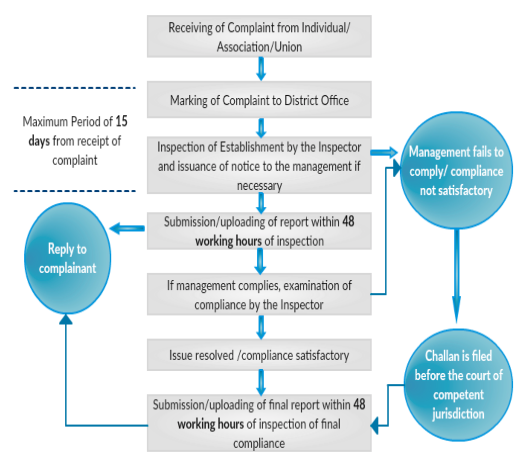
\includegraphics[height = 4.3in]{fig1.png}
\captionsetup{justification=centering}\caption[Optional Caption]{Inspection Procedure Flowchart as Given in the Inspection Checklist by the Delhi Labour Department Website}
\end{figure}

Following each of the aforementioned listed steps are certain requirements. For instance, Step 3, that is the conduct of inspections, necessitates that inspectors know and follow the inspection checklist as provided in the SOPs attached to each of the seven laws. For this, inspectors must know which Acts necessitate an on-site inspection. Similarly, following time frames such as submission of reports within 48 hours of inspection requires that all dates and times be clearly mentioned to monitor case progress. \\

We explore the reality of inspection procedures given in the labour law of Delhi by looking at whether these requirements are met. \\

%================Analysing the Reality of Labour Inspections in Delhi==========================
\section{Analysing the Reality of Labour Inspections in Delhi}\label{sec:2}

Our team set out to better understand the labour inspection procedures, investigate timelines and determine how we could objectively analyse the effectiveness of labour inspections in correcting labour malfeasance. In order to study the implementation of the inspection checklist in the New Delhi District Labour Office, we did three things:

\begin{itemize}
\item We assembled administrative data from complaint registers and case files and analysed it against SOP requirements or good practices in inspections.
\item We conducted semi-structured interviews with the Additional Labour Commissioner, Labour Officer, Inspecting Officer and Inspector of the New Delhi district office.\footnote{The post of an inspector is a group C post, while that of an inspecting officer is a group B post. Their jobs remain the same but there is a difference in salary, seniority and mode of recruitment. Inspectors are recruited through Delhi Subordinate Services Selection Board, while inspecting officers are recruited through Staff Selection Board.}
\item We interviewed 15 complainants asking them about the kinds of problems they faced with the inspection process and their satisfaction with the process. We found the names and contact details of these complainants from complaint registers. The questionnaire for these interviews is provided in Appendix 2. 
\end{itemize}

In this study we have not reached out to enterprises named in the complaints. 

%Administrative Records Analysis of Labour Violation Complaints Data
\subsection{Administrative Records Analysis of Labour Violation Complaints Data}

Every complaint received is supposed to have an entry into the complaint register along with the detailed case file. We were granted access to four such complaint registers and 20 such case files maintained by the New Delhi District Labour Office. To our knowledge, this is the first study that systematically looks at administrative data from complaint registers and case files to understand procedural hygiene in complaint resolution. \\

%Tabulation and Study of Complaint Registers
\subsubsection{Tabulation and Study of Complaint Registers}

The complaint register is a record of all the complaints received by the office. It consists of 
\begin{itemize}
\item names and addresses of complainants; 
\item important dates (complaint receipt, hearings, settlement); 
\item the Acts under which individual complaints were registered; 
\item whether the case was settled.\footnote{Settlement means that either the complaint was resolved or it was forwarded to the court of appropriate jurisdiction.} \footnote{Some cases don’t get settled but are simply closed from the inspector’s end as complainants stop responding. Date of closure does not indicate whether the case was settled or not.} 
\end{itemize}
 
A total of 846 complaints were filed between 1 January 2016 and 11 July 2018 in the registers provided to us. Table 3 shows how we tabulated all the 846 complaints. The actual register includes other parameters such as the name, address, and phone number of the complainant, which we omitted from our tabulation. \\

%Table 3: Sample Tabulation of Administrative Data from Complainant Register
\begin{table}[H]
\caption{Sample Tabulation of Administrative Data from Complainant Register}
\begin{tabular}{L{3cm}L{1.7cm}C{3cm}C{3cm}C{3cm}}
\toprule
Act & Settled & \multicolumn{3}{c}{Relevant Dates} \\
\midrule
& & \textit{\footnotesize{Receipt of Complaint}}	&	\textit{\footnotesize{First Day of Hearing}} & \textit{\footnotesize{Resolution or Closure}}\\
\midrule
			$-$	&	Yes		&	01/01/2016	&	11/01/2016		&		11/03/2016\\
			$-$	&	Yes		&	$-$		&	05/02/2016	&		05/02/2016\\
			$-$	&	No		&	05/01/2016	&	27/05/2016	&	$-$\\
			Minimum Wages Act, 1948	&	Yes		&	08/01/2016	&18/01/2016	&	$-$\\
\bottomrule
\end{tabular}
\end{table}

Not all parameters were uniformly entered in the registers. As a result, each finding in our analysis was based on a unique usable dataset of register entries for which the relevant information was entered in the register. For example, to calculate the time taken to resolution, we used entries that included dates for receipt of complaints and available dates of resolution. Our tabulation of entries in the complaint registers and data analysis is available in Appendix 3 for reference.

%Study of Case Files
\subsubsection{Study of Case Files}
Each complaint in the registers had a separate case file. We analysed 20 such case files. \\

A case file consists of all the documentation provided by the establishment and past correspondence between the inspectorate, the complainants and the establishment for that one complaint. Case files typically include: 
\begin{itemize}
\item the original complaint (received in the form of a letter); 
\item the notices issued by the inspector to the management; 
\item notes from any correspondence between the inspector, complainant and management; 
\item written responses of the management to the notice from the inspector;
\item a copy of the challan (charge sheet), if filed. (Filling the challan means that the case has been forwarded to the appropriate court for resolution.)
\end{itemize}

In the next section, we present our findings from the analysis of these 846 unique complaints and findings from interviews with the New Delhi District Labour Office officials and complainants. We acknowledge that administrative data accuracy relies on the ability of the inspector to input the data accurately and honestly.  

%================Actual Procedural Hygiene of Labour Compliance Enforcement in New Delhi=======
\section{Actual Procedural Hygiene of Labour Compliance Enforcement in New Delhi}\label{sec:3}

Through our analysis of administrative data on complaints and through interviews with inspecting officers and complainants, we find that while SOPs have been published on the website of the department, they are likely not being met with rigour. We estimate that the labour complaint resolution process in Delhi falls short of meeting best practice standards in several areas. 
\begin{enumerate}
\item Indifferent, haphazard and nonstandardised record keeping and lack of fidelity to prescribed timelines are nontrivial departures from SOPs or best practices.
\item The high number of cases pending resolution may be highlighting a deeper malaise with the redressal mechanism because more than half of the complaints we analysed remain unsettled for almost a year.\footnote{In the complaint register that we analysed, the inspector had marked ‘Settled’ for the complaints that were settled. The inspector, however, did not mark any complaint as not settled. Therefore, we assumed that any complaints not marked ‘settled’ have not been settled till date.}
\item The resolution process relies on inspections and hearings which are not defined in SOPs. This has likely made inspections vulnerable to ‘window dressing’.
\item Complainants remain dissatisfied with the redressal mechanism. Most complainants emphasise collusion between department officials and plaintiff representatives. 
\item Contrary to claims by department officials that manpower shortages are the key reason for poor procedural hygiene, high pendency and complainant dissatisfaction, we estimate that low levels of awareness among inspectors about the laws and blurry lines between on-site inspections and in-office hearings may be contributing to these poor outcomes. 
\end{enumerate}

%Indifferent and Inconsistent Record Keeping 
\subsection{Indifferent and Inconsistent Record Keeping}

\textbf{Requirement:} No requirement and no prescribed format given for how labour inspectors should maintain registers.\\

\textbf{Reality:}  Since there is no prescribed format or mandate for record keeping, we find that registers and case files have been maintained in an inconsistent manner. \\

Record keeping is a matter of policy and good administrative practice developed over time and built into work processes to ensure that the organisation can refer to records of past transactions. This aids organisations to perform subsequent actions, produce evidence of financial or contractual obligations and avoid disputes or protect against legal liability. It also helps draw on evidence of past events to make informed decisions for the present and future. Good record keeping practices allow organisations to account for their actions and decisions when required to do so. \\

Labour inspectors have access to very valuable information given their interactions with the management, visit workplaces and access to the records of the establishment. In order to fully utilise this information, it should be collected in accordance with certain guidelines, principles and methodologies (\cite{iloreportstatistics}, 1). In fact, if labour inspectorates record the data required for administrative purposes methodologically and uniformly, the data can help in the diagnosis of issues and the design of responses to priority problems (\cite{iloreportstatistics}, 2). \\

The procedure for inspections and resolution of complaints entails maintenance of complaint registers and preparation of individual case files. Both these at the New Delhi District Labour Office are poorly maintained. \\

Case files are supposed to contain proof of all correspondence between the complainant, the employer and the inspector. Case files typically include the original complaint (received in the form of a letter), notices issued by the inspector to the management, notes from any telephonic correspondence between the inspector, the complainant and the management, letter responses of the management to the notice from the inspector and a copy of the challan if filed. Filing of the challan means that the case has been forwarded to the court of appropriate jurisdiction for resolution. \\

For the 20 case files we analysed, we found several documents missing from the files. These case files were assigned to us by the inspectors. Thus, one can presume that these case files were the least controversial ones. Some cases had the copy of the first notice missing, while some case files did not have the complaint letter to begin with. \\

Complaint registers are also poorly maintained. They are currently handwritten and manually maintained, which reduces their accessibility. Our visit to the New Delhi District Labour Office revealed that the inspector at the district did not even have a computer. \\
 
In the absence of a prescribed format or method for entering information in registers, there was no uniformity in tabulation between the complaint registers we analysed. For example, one of the four complaint registers mentioned all the dates of inspections/hearings while the other three only mentioned the date of first hearing. The writing was illegible and complaints were not recorded in a standardised language. The complaints were written in either Hindi or English. \\

The five parameters that we used to tabulate the data from the complaint registers had missing information. For 781 out of 846 complaints the \textbf{Act} they were filed under was missing. The \textbf{date of receipt of a complaint} for 63 out of 846 complaints, \textbf{date of first hearing} for 166 out of 846 complaints and \textbf{date of resolution} for 89 out of 382 resolved cases had not been mentioned. For all 846 complaints it was said if they had been settled or not. Table 4 shows just how poorly the registers are compiled and maintained. 



%Table 4: Analysis of Complaints in the Four Complaint Registers of the New Delhi District Labour Office
\small
\begin{longtable}[l]{>{\raggedright}p{8cm}>{\centering\arraybackslash}p{6.5cm}}
\caption{Analysis of Complaints in the Four Complaint Registers of the New Delhi District Labour Office}\\
\toprule
Parameter &  Findings \\
\midrule
Number of complaints in the register & 846 \\
 & \\
Missing complaint dates & 7.4\% \\
 & \\
Missing first hearing dates & 19.6\% \\
 & \\
Missing closure dates & 23.3\%\\
 & \\
Missing Act of the registered complaint & 92.3\% \\
\midrule
 \multicolumn{2}{c}{Other Findings from the Registers} \\
\midrule
\multicolumn{2}{l}{\footnotesize{• 98.5\% of the cases in the registers had at least one or the other field with missing information.}} \\
\multicolumn{2}{l}{\footnotesize{• Of the 20 case files we studied, one-fourth (25\%) had no mention in the registers.}} \\
\multicolumn{2}{l}{\footnotesize{• In 12 complaints from the registers, the date of hearing was after the date of receipt of }}\\ \multicolumn{2}{l}{\footnotesize{the complaint.}} \\
\multicolumn{2}{l}{\footnotesize{• In 6 complaints from the register, the date of closure was before the date of receipt.}} \\
\multicolumn{2}{l}{\footnotesize{• In 3 complaints, the date of receipt is after 11 July 2018–the date when we analyzed}}\\ \multicolumn{2}{l}{\footnotesize{the registers.}} \\
\multicolumn{2}{l}{\footnotesize{• Complaint records are not written in a standardized language.}} \\
\multicolumn{2}{l}{\footnotesize{• The order of sections in the four registers were different. There were differences even }}\\
\multicolumn{2}{l}{\footnotesize{within the same register as documentation format changed month to month. }} \\
\bottomrule
\end{longtable}
\normalsize


All of the problems mentioned in the aforementioned table could potentially be avoided through a standardised system of record keeping. 

%Lack of Fidelity to Prescribed Timelines
\subsection{Lack of Fidelity to Prescribed Timelines}

\textbf{SOP Requirement:} According to the inspections checklist on the Delhi Labour Department website, inspections have to be conducted within 15 days of receipt of complaint.\\

\textbf{Reality:} We find that inspections timelines are regularly not met.\\

Under the complaint redressal system, labour inspectors are supposed to carry out inspections within 15 days of receipt of complaint; and inspection reports should be submitted to a higher authority or uploaded online within 48 hours of inspection \parencite{inspectionsop}. We find that in 33.6\% cases inspections were held after 15 days of receipt of complaints, with the average time between receipt of complaint and first hearing being 16.8 days (See Table 5). 

%Table 5: Compliance with Timelines for Resolution of Complaints
\small
\begin{longtable}[l]{>{\raggedright}p{5.5cm}>{\raggedright}p{4.5cm}>{\centering\arraybackslash}p{4.5cm}}
\caption{Compliance with Timelines for Resolution of Complaints}\\
\toprule
Parameter & Number of observations which had relevant timelines & Findings \\
\midrule
Inspections held after required 15 days of receipt of complaint
 & 612/846 cases\footnotemark & 33.6 \% \\
 & \\
Average time from receipt of complaint till first hearing & 612/846 cases & 16.8 days (more than the mandated 15 days.)\\
\hline
 \multicolumn{3}{c}{Other Findings} \\
\midrule
\multicolumn{3}{l}{\footnotesize{• Although inspectors maintain handwritten reports as a part of case files, interviews with}}\\ \multicolumn{3}{l}{\footnotesize{inspectors illustrated that inspectors are unaware of the provision requiring submission of}}\\ \multicolumn{3}{l}{\footnotesize{inspection reports to senior officers within 48 hours.}} \\
\bottomrule
\end{longtable}
\normalsize
\footnotetext{Only 612 out of 846 entries in the registers had information about complaint dates and first hearing dates.}

Delay in the resolution of these complaints causes heightened distrust in the inspectors, as disclosed by complainants in interviews. \\

We have no information about whether the final reports are submitted within 48 hours of conducting the inspection or not. Recommendations C and D of the BRAP, which mandate submission of reports online and allow establishments to download reports, were never adopted by the Government of Delhi Complainants mentioned during the interview how they were unaware whether the inspector played any part at all in resolving their complaints because they did not have access to the inspection reports. \\

Timely reports can help formulate effective inspection policies, while also providing proof of proceedings (\cite{iloreportamerica}). The report should be completed as soon as possible after the inspection, preferably on the same day. There should ideally be binding deadlines throughout the inspectorate with clear, achievable performance standards. Timely submission of reports to a higher authority leads to increased accountability, which improves performance.

%High Number of Cases Pending Settlement
\subsection{High Number of Cases Pending Settlement}

\textbf{Requirement:} No given time frame within which cases should be settled.\\

\textbf{Reality:} In a system with no given time frame for complaint resolution, 54.8\% of the cases have been left unresolved for an average of 311.5 days.\\

There are time frames provided in the labour inspections checklist for steps in the inspection process, such as date till inspection and submission of reports. There is, however, no time frame mentioned for cases to be settled/resolved. A case is only settled/resolved if the complaint has been resolved by the inspector or the complaint has been forwarded to the appropriate court for further action. For 2016–2018 in New Delhi, 55.9\% of the cases have been unresolved for an average of 311.5 days for the 436 cases that have not been settled.\footnote{Settled here means that either the complaint was resolved by the inspector or it was forwarded to the appropriate court for further action.} The 260 cases that had been settled took an average time of 43.6 days. This is an interesting relationship because the cases that got settled were resolved fairly quickly compared with the unresolved cases.\\

Table 6 illustrates the failure of the complaint redressal system to settle complaints. Here, we see the implications of the neglect of deadlines of conducting an inspection within 15 days of receipt of complaint.

%Table 6: Discrepancies in Resolution of Labour-Related Complaints
\small
\begin{table}[H]
\caption{Discrepancies in Resolution of Labour-Related Complaints}
\begin{tabular}{L{6cm}C{5cm}C{3cm}}
\toprule
Parameters & Usable Data & Findings\\
\midrule
Unsettled cases & 846 cases & 54.8\%\\
Average time taken to solve complaints & 260 settled cases\footnotemark & 43.6 days\\
Average time since receipt of complaint & 438 unsettled cases & 311.5 days\\
\midrule
\multicolumn{3}{c}{Other Findings}\\
\midrule
\multicolumn{3}{p{15cm}}{\textbf{Of the 15 complainant interviewed, about half claimed that their \newline complaints were yet to be unresolved:}}\\
\multicolumn{3}{p{15cm}}{\footnotesize{•25\% of the complainants who were yet to see resolution were harassed by the management and, therefore, did not pursue their complaints.}}\\
\multicolumn{3}{p{15cm}}{\footnotesize{•The other 75\% have been waiting for an average of 161 days since the date of receipt of complaint by the Delhi Labour Department  for resolution as of 16 July 2018 (the date of the interviews).}}\\
\multicolumn{3}{p{15cm}}{\footnotesize{•Meanwhile, the 47\% of complaints that did get resolved, were done so in 35 days on average.}}\\
\bottomrule
\end{tabular}
\end{table}
\footnotetext{The two numbers do not add to the total of 846 cases because of the presence of unusable data.}
\normalsize

%Confusion Between ‘Inspection’ and ‘Hearing’ in the Absence of a Clear Definition
\subsection{Confusion Between ‘Inspection’ and ‘Hearing’ in the Absence of a Clear Definition}

\textbf{SOP Requirement:} On-site inspections are required for five out of the seven labour Acts mentioned in the BRAP reforms. No prescribed format of redressing complaints of the other two Acts exists. \\

\textbf{Reality:} Less than 10\% of the complaints are registered under the five Acts which require on-site inspections, and even in those cases on-site inspections are hardly ever conducted. For the other cases, an informal system of summoning the management and the employee to the Labour Office is followed.\\
 
On-site inspections provide a way for inspectors to triangulate complaints. On-site inspections in New Delhi, however, are hardly ever conducted. In most cases, the establishments are simply called to the Labour Office to redress the complaint. \\

In our analysis of the 20 case files, we came across only 2 complaints where an on-site inspection was carried out. Our basis for concluding that an inspection was carried out for these two cases is the existence of the photocopy of the inspection report in these two files. Additionally, when we asked the labour officer to show us any case file in which case an on-site inspection was conducted, they could not find any. \\

Under the complaint redressal system, labour inspectors are required to conduct on-site inspections in all cases, except for complaints under the Payment of Bonus Act, 1965, and the Minimum Wages Act, 1948. From the 48 complaints filed in 2018\footnote{Registers for 2016 and 2017 did not have a column for acts. We, therefore, only look at complaints from the 2018 register.} which did have the Act mentioned, 93.6\% of the complaints were under either the Minimum Wages Act, 1948, or the Payment of Bonus Act, 1965. As a result, inspectors mostly summon the management of the concerned establishment to the respective district office, where the relevant records are produced for inspection. \\

One of the key disadvantages of such an inspection process is ‘window dressing’ and documents being ‘missing’ \parencite{iloreportlabour}. Moreover, this system of calling the management to the Labour Office is not mentioned in either the inspection checklist or the Acts. As a result, there is no prescribed format. It is unclear what the due process is and whether it is followed. 

%Dissatisfaction Among Complainants with Inspections and Resolution Process
\subsection{Dissatisfaction Among Complainants with Inspections and Resolution Process}

Interviews with the complainants revealed that 40\% of the complainants were not satisfied with the complaint redressal system.\\ 
Complainants cited various causes of dissatisfaction: harassment from the management of the concerned establishment; the management not appearing at the hearing; failure of the inspector to furnish the final inspection report to the complainant; and close proximity between the labour inspector and establishment resulting in a bias against the complainant. Complainants faced challenges when filing the complaints because of lack of awareness. For example, complainants were not able to gain access to inspection reports or had to pay a fee to file their complaint.\\

Where complainants claimed that their case was a pending resolution, an average of 161.25 days had elapsed since registering the complaint. Where complaints were resolved, complainants stated that it took about 35 days on average.\\

Table 7 illustrates our findings from the complainant interviews we conducted.

%Table 7: Findings from Complainants
\begin{table}[H]
	\caption{Findings from Complainants}
	\begin{tabular}{L{10cm}C{4cm}}
	\toprule
	Parameter & Findings (\%)\\
	\midrule
	Complainants who met the inspector\footnotemark & 87\\
	Complainants who faced problems with filing of complaint. & 54\\
	Satisfaction with the Complaint Redressal system & 40\\
	Complainants who claimed to be harassed by Management & 60\\
	Complainants that claimed Inspector was not proactive & 40\\
	Complainants who viewed their complaint to be unresolved & 47\\
	\bottomrule
	\end{tabular}
\end{table}
\footnotetext{One of the complainants did not meet the inspector because she resolved the complaint with the management and one reported that the labour court was not responsive.}

Complainants argue that there is close proximity between the management and the inspectors, which allows the management to window dress their records and files and is prone to corruption. Since inspectors are aware that it makes economic sense for employers to compromise with the monitors of laws rather than implement them, they make extortionist demands that employers comply with \parencite{hindunews2}. The complaint redressal mechanism, as in force today, leaves a large degree of discretion at the hands of the inspectors and thereby encourages corruption and rent seeking \parencite{debroynews}. 

%Other Issues
\subsection{Other Issues}
%Lack of Awareness Among Inspectors
\subsubsection{Lack of Awareness Among Inspectors}

\textbf{Requirement:} Inspectors are required to know what constitutes violations of labour laws in order to follow the SOPs for each Act. \\

\textbf{Reality:} During interviews, inspectors demonstrated a lack of knowledge about what constitutes the violation of labour laws such as the Equal Remuneration Act.\\

We went beyond our analysis of the complaint register and the case files to find how well the primary enforcers of labour laws, ‘the inspectors’, know the various labour laws. To our dismay, we found through our interviews with the inspectors that they were unaware about the crucial provisions of labour laws. \\

For example, labour inspectors seemed unaware about discrimination clauses of the Equal Remuneration Act, 1976. When asked how they judge discrimination under the Act, inspectors claimed that discrimination during promotion did not come under the Act. However, Section 5 of the Equal Remuneration Act, 1976, clearly states that discrimination during recruitment/promotion is a violation. The Additional Labour Commissioner claimed that the Act was redundant because there had not been any cases under it in the last 25 years. This claim, however, is refuted by the Delhi Labour Department website, which shows that there were 2,826 inspections under the Equal Remuneration Act in 2002 \parencite{officeofthelabourcommissioner}. \\

%Unclear Manpower Planning
\subsubsection{Unclear Manpower Planning}

Delhi Labour Department currently has a large proportion of vacant positions. In order to assess the organisation team strength for 2018, our team visited the office of the Labour Commissioners and accessed data on the number of vacancies in the department through their administrative office (See Table 8). 

%Table 8: Sanctioned and Vacant Positions within the Delhi Labour Department
\begin{longtable}[l]{>{\raggedright}p{4cm}>{\centering}p{3.75cm}>{\centering}p{3cm}>{\centering\arraybackslash}p{2.5cm}}\\
\caption{Sanctioned and Vacant Positions within the Delhi Labour Department}\\
\toprule
Post & Sanctioned Positions & Vacant Positions & Vacancy \% \\
\midrule
Inspecting Officer & 19  & 13 &  68.4\\
Inspector (Grade 2) & 38  & 27 & 71.1 \\
Inspector (Grade 3) & 13 & 9 & 69.2 \\
Labour Officer & 11 & 3 & 27.3 \\
Assistant Labour Commissioner (ALC) & 11 & 0 & 0.0 \\
Deputy Labour Commissioner (DLC) & 13 & 7 & 53.8 \\
Inspector of Factory & 10 & 5 & 50.0 \\
Joint Labour Commissioner (JLC) & 3 & 0 & 0.0\\
\midrule
Total & 118 & 64 & 54.2 \\
\bottomrule
\end{longtable}

There are only 15 inspectors in the Delhi Labour Department spread over nine district offices. Approximately, 83\% of the sanctioned inspector positions remain unfilled. Since 2013, the number of inspectors in the department in Delhi has increased by only 2 \parencite{scroll}. \\

The large number of vacancies, however, does not imply that the Delhi Labour Department is overburdened. This is certainly not the case for the New Delhi District Labour Office. While inspectors at the New Delhi District Labour Office claimed to deal with approximately 60–80 cases per month, our analysis of the complaint register does not support the claim. The complaint register shows that an inspector receives 25.9 complaints a month, which implies approximately 1 complaint per day. Moreover, most complaints received are filed under the Minimum Wages Act, 1948, and the Payment of Bonus Act, 1965, which do not necessitate an on-site inspection as explained earlier.  

%================CONCLUSION=====================================================
\section*{Conclusion}
\addcontentsline{toc}{section}{Conclusion}

The DIPP has employed self-reporting as a method of receiving feedback on progress made in the implementation of reforms by states under the BRAP 2017. Our study highlights the limitations that arise from self-reporting of progress and emphasises the need to critically examine the veracity of claims made with regard to the implementation of reforms and investigate what is not being said. \\

We find that the GoNCT currently handles labour inspections in a rudimentary manner: record keeping is done manually, and inspection reports are not uploaded online. Our preliminary investigation reveals that procedural hygiene in the New Delhi Labour Inspectorate is not up to the mark. \\

Several states in India have employed measures to increase transparency and efficiency in the existing system of inspections. Instead of shifting to a complaint redressal system, the procedure of suo-moto inspections has been improvised. In 2011, the ILO recognised the Labour Management System (LMS) developed by the Government of Maharashtra to facilitate compliance with labour laws. The LMS was designed to streamline the labour machinery of the state by consolidating information gathered from labour inspections and generating automatic alerts to help monitor labour law compliance \parencite{iloreport}. It provides for an online complaint window for businesses and labourers \parencite{bestpractices} and allows users to track their past inspections \parencite{mahaonline}. Moreover, several states, including Andhra Pradesh and Telangana, have developed a portal for employers and employees to download inspection reports \parencite{apgovernment}, thus making the system more transparent.\\

Taking guidance from the BRAP 2017, released by the DIPP, Jharkhand and Andhra Pradesh introduced centralised portals for dealing with inspections. The practice followed in Jharkhand has been listed as the best practice for labour reforms by the DIPP. These systems categorise establishments, randomly allocate establishments to inspectors, display a list of establishments to be inspected and allow employers and employees to access inspection reports.\\

The Delhi Labour Department, however, does not appear to be meeting the intent behind the BRAP 2017 implementation guideline. A regulatory system must be built on the doctrine of rule of law. There should be no opportunities for abuse of power, transparency in all aspects of enforcement, strong challengibility in a court of law and high standards of professional conduct. In Delhi, however, one doesn’t know if due process and procedural hygiene are being adhered to. \\

We asked the complainants about their views on improving the system at play in Delhi and they suggested the following:
\begin{itemize}
\item Labour court proceedings should be conducted in front of a camera so that files and evidence do not get ‘misplaced’ as certain complainants have experienced.
\item Inspectors should retroactively check if the management continues to comply with the laws and have not harassed the workers after the complaint has been settled. 
\item Also, 33.3\% of the complainants recommended that there should be regular inspections rather than complaint-based inspections. CRA, as recommended under Reform E of the BRAP implementation guidelines, is a possible alternative which ensures regular inspections in high-risk areas.
\end{itemize}

Since ‘inspector raj’ is a product of unchecked discretion placed in the hands of the inspectors, self-reporting by these inspectors does not provide us with a clear perspective of progress on eliminating it. The aim of reforming the inspection system is to provide for equal treatment of all, bring in transparency and accountability and put in place a satisfactory complaint redressal mechanism. Mere publishing SOPs on the department websites hardly fulfils the purpose of ease of doing business.

%================BIBLIOGRAPHY====================================================
\newpage
\section*{Bibliography}
\addcontentsline{toc}{section}{Bibliography}
\printbibliography[heading=none]
%================APPENDICES=====================================================
%Appendix 1
\newpage      
\section*{Appendix 1: List of Labour Laws in Force in Delhi}
\addcontentsline{toc}{section}{Appendix 1: List of Labour Laws in Force in Delhi}

\textbf{List of Central Labour Acts}
\setlist{nolistsep}
\begin{enumerate}[noitemsep]
\item The Workmen's Compensation Act, 1923 (now renamed as the Employees Compensation Act, 1923)
\item The Working Journalists and Other Newspapers Employees (Conditions of Service) and Compensation Act, 1923)
\item The Trade Unions Act, 1926
\item The Payment of Wages Act, 1936
\item The Children's (Pledging of Labour) Act, 1938
\item The Employees Liability Act, 1938
\item The Weekly Holidays Act, 1942
\item The Industrial Employment (Standing Orders) Act, 1946
\item The Mica Mines Labour Welfare Fund Act, 1946
\item The Industrial Disputes Act, 1947
\item The Factories Act, 1948
\item The Employees State Insurance Act, 1948
\item The Minimum Wages Act, 1948
\item The Plantation Labour Act, 1951
\item The Employees Provident Fund and Miscellaneous Provisions Act, 1952
\item The Mines Act, 1952
\item Miscellaneous Provisions Act, 1955
\item The Employment Exchange (Compulsory Notification of Vacancies) Act, 1959
\item The Building and Other Construction Workers Cess Act, 1996 
\item The Apprentices Act, 1961
\item The Maternity Benefit Act, 1961
\item The Motor Transport Act, 1961
\item The Personal Injuries (Emergency Provisions) Act, 1962
\item The Personal Injuries (Compensation Insurance) Act, 1963
\item The Payment of Bonus Act, 1965
\item The Beedi and Cigar Workers (Conditions of Employment) Act, 1966
\item The Contract Labour (Regulation and Abolition) Act, 1970
\item The Limestone and Dolomite Mines Labour Welfare Fund Act, 1972
\item The Payment of Gratuity Act, 1972
\item The Sales Promotion Employees (Conditions of Service) Act, 1976
\item The Bonded Labour System (Abolition) Act, 1976
\item The Iron Ore Mines, Manganese Ore Mines and Chrome Ore Mines Labour Welfare Fund Act, 1976
\item The Iron Ore Mines, Manganese Ore Mines and Chrome Ore Mines Labour Welfare (Cess) Act, 1976
\item The Beedi Workers Welfare Fund Act, 1976
\item The Beedi Workers Welfare Cess Act, 1976
\item The Equal Remuneration Act, 1976
\item The Inter-State Migrant Workmen (Regulation of Employment and Conditions of Service) Act, 1979
\item The Cine Workers and Cinema Theatre Workers (Regulation of Employment) Act, 1981
\item The Cine Workers Welfare (Cess) Act, 1981
\item The Cine Workers Welfare Fund Act, 1981
\item The Dock Workers (Safety, Health and Welfare) Act, 1986
\item The Child Labour (Prohibition and Regulation) Act, 1986
\item The Labour Laws (Exemption from Furnishing Returns and Maintaining Registers by Certain Establishments) Act, 1988
\item The Building and Other Constructions Workers' (Regulation of Employment and Conditions of Service) Act, 1996
\item The Unorganised Workers Social Security Act, 2008 \\ 
\end{enumerate}


\textbf{Act Passed by the GoNCT}
\setlist{nolistsep}
\begin{enumerate}[noitemsep]
\item The Delhi Shops \& Establishment Act, 1954
\end{enumerate}

%Appendix 2
\newpage      
\section*{Appendix 2: Questionnaire for \\ Complainant Interviews}
\addcontentsline{toc}{section}{Appendix 2: Questionnaire for Complainant Interviews}

\setstretch{1}
\begin{table}[H]
\begin{mdframed}[backgroundcolor=gray!20]
	\begin{tabular}{L{10cm}L{4cm}}
	%table heads
	%\midrule
	Did the inspector ever meet you? & Yes/No/Other\\
	Was the inspector proactive in solving your complaint? & Yes/No/Other\\
	What problems did you face in filing the complaint? How much money did it cost? & -\\
	Did you pay a bribe to expedite the case? & Yes/No/Other\\
	How long did it take to solve your complaint? & -\\
	What is the current status of your complaint? & -\\
	Are you satisfied by the resolution of the complaint? & Yes/No\\
	Are you satisfied with the process of the complaint-resolving mechanism? & 
	Yes/No\\
	Did you face any kind of harassment for filing of the complaint? & Yes/No/Maybe\\
	 If yes, did you inform of the same to the inspector? & Yes/No/Maybe\\
	 How do you think the system can be improved? (Will regular/periodic inspections prove useful?) &  \\
	\end{tabular}	
	\end{mdframed}
\end{table}

%Appendix 3
\newpage      
\section*{Appendix 3: Database and Analysis of Register Data and Case Files}
\addcontentsline{toc}{section}{Appendix 3: Database and Analysis of Register Data and Case Files}

\textbf{Database Link:} 
http://bit.ly/2EBOJU1 \\ 


\textbf{Data Analysis Link:} 
http://bit.ly/2ys71BC

\end{document}